\tikzset{
	main/.style={black, line width=0.4mm, opacity=1},
	second/.style={gray, opacity=5},
	arrow/.style={-latex, shorten >=1ex, shorten <=1ex, bend angle=45}
}
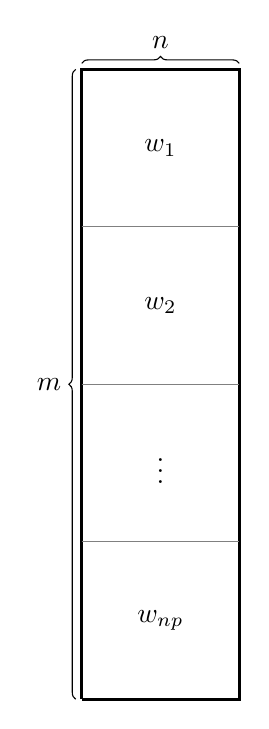
\begin{tikzpicture}
\draw[main] (0,0) -- (2,0) -- (2,8)-- (0,8)-- (0,0);

\draw[second] (0,2) -- (2,2) ;
\draw[second] (0,4) -- (2,4) ;
\draw[second] (0,6) -- (2,6) ;


\draw[decorate, decoration={brace,mirror}, yshift=.5ex]  (2,8) -- node[above=0.4ex] {$n$}  (0,8);
\draw[decorate, decoration={brace}, xshift=-.5ex]  (0,0) -- node[left=0.4ex] {$m$}  (0,8);

\draw (1,7) node {$w_1$};
\draw (1,5) node {$w_2$};
\draw (1,3) node {$\vdots$};
\draw (1,1) node {$w_{np}$};


\end{tikzpicture}